\lab{Importance Sampling and Monte Carlo Simulations}{Importance Sampling and Monte Carlo Simulations}
\objective{Use importance sampling to reduce the error and variance of Monte Carlo Simulations.}
\label{lab:montecarlo2}

\section*{Introduction}

The traditional methods of Monte Carlo integration as discussed in the previous lab are not always the most efficient means to estimate an integral. For example, assume we were trying to find the probability that a randomly chosen variable $X$ from the standard normal distribution is greater than $3$. We know that one way to solve this is by solving the following integral:

\begin{equation} \label{eq:integral} 
P(X > 3) = \int_{3}^{\infty} f_X(t)\,dt = \frac{1}{\sqrt{2\pi}}\int_{3}^{\infty} e^{-t^2/2}\,dt
\end{equation}

If we define the function $h: \mathbb{R} \rightarrow \mathbb{R}$ as 

$$h(t) = \begin{cases}
1 & \text{ if } t > 3 \\ 
0 & \text{ if } t \leq 3 
\end{cases}, $$
we can rewrite this integral as

\begin{equation*}
\int_{3}^{\infty} f_X(t)\,dt = \int_{-\infty}^{\infty} h(t)f_X(t)\,dt.
\end{equation*}

By the Law of the Unconscious Statistician (see Volume 2 \S 3.5), we can restate the integral above as

$$\int_{-\infty}^{\infty} h(t)f_X(t)\,dt = E[h(X)].$$
Being able to write integrals as expected values is an essential tool in this lab.

\section*{Monte Carlo Simulation}
In the last section, we expressed the probability of drawing a number greater than $3$ from the normal distribution as an expected value problem. We can now easily estimate this same probabilty using Monte Carlo simulation. 
Given a random i.i.d. sample $x_1, x_2, \cdots , x_N$ generated by $f_X$, we can estimate $E[h(X)]$ using
\begin{equation} \label{eq:estimator}
\widehat{E}_n[h(X)] = \frac{1}{N}\sum_{i = 1}^{N}h(x_i)
\end{equation}

Now that we have defined the estimator, it is now quite manageable to approximate Equation \ref{eq:integral}. By the Weak Law of Large Numbers (see Volume 2 \S 3.6), the estimate will get closer and closer to the actual value as we use more and more sample points.

\begin{comment}
\begin{lstlisting}
>>> h = lambda x : x > 3
>>> N = 10**7
>>> x = np.random.normal(size=N)
>>> 1./N * np.sum(h(x))
0.0013644
\end{lstlisting}
\end{comment}

\begin{problem} \label{prob:mc}
Write a function in Python that estimates the probability that a random draw from the standard normal distribution is greater than 3 using Equation \ref{eq:estimator}. Your function should accept a parameter \li{n} for the number of samples to use in your approximation. Your answer should approach $0.0013499$ for sufficiently large samples.
\end{problem}

Though this approach gets the job done, it turns out that this isn't very efficient. Since the probability of drawing a number greater than $3$ from the standard normal distribution is so unlikely, it turns out we need many sample points to get a good approximation.

\section*{Importance Sampling}
Importance sampling is one way to make Monte Carlo simulations converge much faster. We choose a different distribution to sample our points to generate more \emph{important} points. With our example, we want to choose a distribution that would generate more numbers around $3$ to get a more reliable estimate. The theory behind importance sampling boils down to the following result. In these equations, the random variable $X$ is generated by $f_X$ and the random variable $Y$ is generated by $g_Y$. We will refer to $X$ and $Y$ in this way for the remainder of the lab.

\begin{equation} \label{eq:importance}
\begin{split}
E[h(X)] & = \int_{-\infty}^{\infty} h(t)f_X(t)\,dt \\
& = \int_{-\infty}^{\infty} h(t)f_X(t)\left ( \frac{g_Y(t)}{g_Y(t)} \right )\,dt \\
& = \int_{-\infty}^{\infty} \left ( \frac{h(t)f_X(t)}{g_Y(t)} \right )g_Y(t)\,dt \\
& = E\left [ \frac{h(Y)f_X(Y)}{g_Y(Y)}\right ]
\end{split}
\end{equation}

The corresponding estimator is

\begin{equation}\label{eq:imp_estimator}
\begin{split}
\widehat{E}[h(X)] & = \widehat{E}\left [ \frac{h(Y)f_X(Y)}{g_Y(Y)}\right ] \\
& = \frac{1}{N}\sum_{i = 1}^{N}\frac{h(y_i)f_X(y_i)}{g_Y(y_i)}
\end{split}
\end{equation}

The function $f_X$ is the p.d.f. of the \emph{target distribution}. The function $g_Y$ is the p.d.f. of the \emph{importance distribution}. The fraction $\frac{f_X(X)}{g_Y(X)}$ is called the \emph{importance weight}. This allows us to draw a sample from any distribution with p.d.f. $g_Y$ as long as we multiply $h(X)$ by the importance weight. 

\subsection*{Choosing the Importance Distribution}
There is no correct choice for the importance distribution. It may be possible to find the distribution that allows the simulation to converge the fastest, but oftentimes, we don't need a perfect answer. Close to perfect is good enough.

We will solve the same problem as in Problem \ref{prob:mc} using importance sampling. We will choose $g_Y$ to be the normal distribution with $\mu = 4$ and $\sigma = 1$. 
We have chosen this distribution for $g_Y$ because it will give us more points closer to and greater than 3. Note that it is not necessary to choose an importance distribution of the same type.

\begin{figure}[H]
\includegraphics[width=\textwidth]{importance_distribution.pdf}
\caption{In our problem, we choose an importance distribution that will generate more samples that are greater than 3. Though not a perfect choice, choosing a normal distribution with $\mu = 4$ and $\sigma = 1$ will suffice.}
\label{fig:importance}
\end{figure}

\begin{lstlisting}
>>> import scipy.stats as stats
>>> h = lambda x : x > 3
>>> f = lambda x : stats.norm().pdf(x)
>>> g = lambda x : stats.norm(loc=4,scale=1).pdf(x)

# Sample from the N(4,1).
>>> N = 10**7
>>> X = np.random.normal(4,scale=1,size=N)

# Calculate estimate.
>>> 1./N * np.sum(h(X)*f(X)/g(X))
0.00134921134631
\end{lstlisting}

\begin{figure}[H]
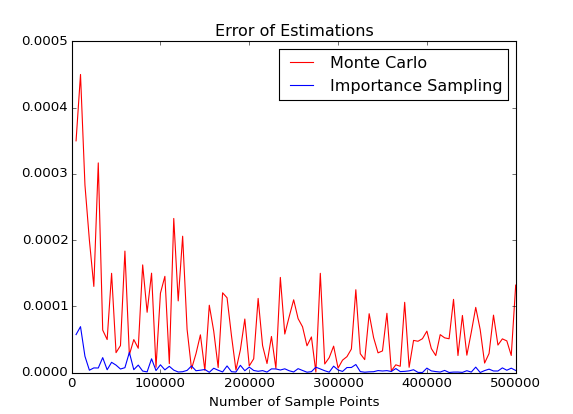
\includegraphics[width=\textwidth]{MCvsIS.png}
\caption{Comparison of error between standard method Monte Carlo and Importance Sampling method of Monte Carlo.}
\label{fig:compare}
\end{figure}

\begin{problem} \label{prob:gamma}
A tech support hotline receives an average of 2 calls per minute. What is the probability that they will have to wait at least 10 minutes to receive 9 calls? Implement your estimator using importance sampling. Calculate estimates using 5000, 10000, 15000, $\cdots$, 500000 sample points. Return an array of estimates. Your answers should approach $0.00208726$. 

Hint: In Volume 2 \S 3.5, the gamma distribution is defined as, $$f_X(x) = \frac{b^{a}x^{a-1}e^{-xb}}{\Gamma(a)}.$$ The version of the gamma distribution in \li{scipy.stats} is determined by the shape ($a$) and the scale ($\theta$) of the distribution. $$f_X(x) = \frac{x^{a-1}e^{-x/\theta}}{\Gamma(a)\theta^a}$$
You can switch between these representations this with the fact that $\theta = 1/b$.
\end{problem}

\begin{problem}
In this problem, we will visualize the benefits of importance sampling. Create a plot of the error of the traditional methods of Monte Carlo integration and the importance sampling methods of Monte Carlo for Problem \ref{prob:gamma}. What do you observe? Your plot should resemble Figure \ref{fig:compare}.

Hint: The following code solves Problem \ref{prob:gamma} using traditional methods of Monte Carlo integration:
\begin{lstlisting}
h = lambda x : x > 10
MC_estimates = []
for N in xrange(5000,505000,5000):
    X = np.random.gamma(9,scale=0.5,size=N)
    MC = 1./N*np.sum(h(X))    
    MC_estimates.append(MC)
MC_estimates = np.array(MC_estimates)
\end{lstlisting}

Hint: To determine the error of your approximations, the following code returns the actual value of the probability:
\begin{lstlisting}
1 - stats.gamma(a=9,scale=0.5).cdf(10)
\end{lstlisting}
\end{problem}

Now that we have visualized the benefits of importance sampling, note that we can achieve the same results as traditional Monte Carlo with a fraction of the samples.

\section*{Generalizing the Principles of Importance Sampling}
The examples we have explored to this point in the lab were merely educational. Since we have a simple means of calculating the correct answer to Problem \ref{prob:gamma}, it doesn't make much sense to use methods of Monte Carlo in this situation. However, as discussed in the previous lab, there are not always closed-form solutions to the integrals we want to compute.

We can extend the same principles we have discussed thus far to solve many types of problems. For a more general problem, we can implement importance sampling by doing the following:
\begin{enumerate}
\item Define a function $h$ where, $h(t) = \begin{cases}
1 & \text{ if condition is met }  \\ 
0 & \text{ otherwise}
\end{cases} $.  
\item Define a function $f_X$ which is the p.d.f. of the target distribution. 
\item Define a function $g_Y$ which is the p.d.f. of the importance distribution.
\item Use these functions in conjunction with Equation (\ref{eq:imp_estimator}).
\end{enumerate}

\begin{problem}
The joint normal distribution of $N$ independent random variables with mean 0 and variance 1 is
\[
f_X(\x) = \frac{1}{\sqrt{(2 \pi)^N}} e^{-(\x^T\x)/2}.
\]
The integral of $f_X(\x)$ over a box is the probability that a draw from the distribution will be in the box.
However, $f_X(\x)$ does not have a symbolic antiderivative.


\begin{comment}
\item The integral of this function on $B = [-1,1]\times [-1,1]\times[-1,1] \subset \mathbb{R}^3$ can be computed in SciPy with the following code.
\begin{lstlisting}
>>> import scipy.stats as stats

# Define the bounds of the box to integrate over
>>> mins = np.array([-1, -1, -1])
>>> maxs = np.array([1, 1, 1])

# Each variable has mean 0
>>> means = np.zeros(3)

# The covariance matrix of N independent random variables
#    is the NxN identity matrix.
>>> covs = np.eye(3)

# Compute the integral
>>> value, inform = stats.mvn.mvnun(mins, maxs, means, covs)
\end{lstlisting}
Then \li{value} is the integral of $f(\x)$ on $B$.
Use SciPy to integrate $f(\x)$ on $\Omega=[-0.5, 0.75]\times[0,1]\times[0, 0.5]\times[0,1] \subset \mathbb{R}^4$.
\end{comment}

Use what you have learned about importance sampling to estimate the probability that a given random variable in $\mathbb{R}^2$ generated by $f_X$ will be less than -1 in the x-direction and greater than 1 in the y-direction.

Treat $f_X$ as the p.d.f. of your target distribution.
Use the function \li{stats.multivariate_normal} to create a multivariate normal distribution to serve as your importance distribution. 
For more information on how to use this function, consult the documentation for 
\li{stats.multivariate_normal}.
\end{problem}

\section*{Unnormalized Target Densities}
The methods discussed so far are only applicable if the target density is normalized, or in other words, has an integral of 1. If the target density is not normalized, Equation \ref{eq:importance} becomes

\begin{equation*} \label{eq:unnormalized}
\begin{split}
E[h(X)] & = \frac{\int h(t)f(t)\,dt}{\int f(t)\,dt} \\
& = \frac{\int h(t)f(t) \left ( \frac{g_Y(t)}{g_Y(t)} \right )\,dt}{{\int f(t)} \left ( \frac{g_Y(t)}{g_Y(t)} \right )\,dt} \\
& = \frac{\int \left ( \frac{h(t)f(t)}{g_Y(t)} \right ) g_Y(t)\,dt}{\int \left ( \frac{f(t)}{g_Y(t)} \right ) g_Y(t)\,dt} \\
& = \frac{E\left [ \frac{h(Y)f(Y)}{g_Y(Y)}\right ]}{E\left [ \frac{f(Y)}{g_Y(Y)}\right ]}
\end{split}
\end{equation*}

The corresponding estimator becomes
\begin{equation*}
\begin{split}
\widehat{E}_n[h(X)] & = \frac{\widehat{E}\left [ \frac{h(Y)f(Y)}{g_Y(Y)}\right ]}{\widehat{E}\left [ \frac{f(Y)}{g_Y(Y)}\right ]} \\
& = \frac{\frac{1}{N}\sum_{i = 1}^{N}\frac{h(y_i)f(y_i)}{g_Y(y_i)}}{\frac{1}{N}\sum_{i = 1}^{N}\frac{f(y_i)}{g_Y(y_i)}} \\
\end{split}
\end{equation*}
